
\documentclass[10pt,a4paper,twocolumn,twoside]{article}
\usepackage[utf8]{inputenc}
\usepackage[catalan]{babel}
\usepackage{multicol}
\usepackage{graphicx}
\usepackage{fancyhdr}
\usepackage{times}
\usepackage{titlesec}
\usepackage{multirow}
\usepackage{lettrine}
\usepackage{hyperref}
\usepackage[top=2cm, bottom=1.5cm, left=2cm, right=2cm]{geometry}
\usepackage[figurename=Fig.,tablename=TAULA]{caption}
\usepackage{svg}
\captionsetup[table]{textfont=sc}

\author{\LARGE\sffamily Pau Casacuberta Orta}
\title{\Huge{\sffamily Disseny d'un ``core'' RISC-V Didàctc}}
\date{}

\newcommand\blfootnote[1]{%
  \begingroup
  \renewcommand\thefootnote{}\footnote{#1}%
  \addtocounter{footnote}{-1}%
  \endgroup
}

%
%\large\bfseries\sffamily
\titleformat{\section}
{\large\sffamily\scshape\bfseries}
{\textbf{\thesection}}{1em}{}

\begin{document}

\fancyhead[LO]{\scriptsize Pau Casacuberta Orta: Disseny d'un ``core'' RISC-V Didàctc}
\fancyhead[RO]{\thepage}
\fancyhead[LE]{\thepage}
\fancyhead[RE]{\scriptsize EE/UAB TFG INFORMÀTICA: Disseny d'un ``core'' RISC-V Didàctc}

\fancyfoot[CO,CE]{}

\fancypagestyle{primerapagina}
{
   \fancyhf{}
   \fancyhead[L]{\scriptsize TFG EN ENGINYERIA INFORMÀTICA, ESCOLA D'ENGINYERIA (EE), UNIVERSITAT AUTÒNOMA DE BARCELONA (UAB)}
   \fancyfoot[C]{\scriptsize Febrer de 2020, Escola d'Enginyeria (UAB)}
}

%\lhead{\thepage}
%\chead{}
%\rhead{\tiny EE/UAB TFG INFORMÀTICA: TÍTOL (ABREUJAT SI ÉS MOLT LLARG)}
%\lhead{ EE/UAB \thepage}
%\lfoot{}
%\cfoot{\tiny{February 2015, Escola d'Enginyeria (UAB)}}
%\rfoot{}
\renewcommand{\headrulewidth}{0pt}
\renewcommand{\footrulewidth}{0pt}
\pagestyle{fancy}

%\thispagestyle{myheadings}
\twocolumn[\begin{@twocolumnfalse}

%\vspace*{-1cm}{\scriptsize TFG EN ENGINYERIA INFORMÀTICA, ESCOLA D'ENGINYERIA (EE), UNIVERSITAT AUTÒNOMA DE BARCELONA (UAB)}

\maketitle

\thispagestyle{primerapagina}
%\twocolumn[\begin{@twocolumnfalse}
%\maketitle
%\begin{abstract}
\begin{center}
\parbox{0.915\textwidth}
{\sffamily
\textbf{Resum--}
Aquest document conté un projecte final de grau on es detalla el disseny a nivell RTL, el procediment de desenvolupament i la implementació en físic d'un processador basat en l'arquitectura RISC-V de 32 bits. Per seguir la filosofia d'Open Hardware i Software. Aquest disseny té la peculiaritat que està pensat per a un entorn didàctic. Això provoca que s'hagi reduït la complexitat del mateix utilitzant el repertori RV32I que només permet fer operacions aritmeticològiques bàsiques amb nombres enters. Tampoc té técniques avançades d'execució, com pipeline o predicció de salts, per reduir la complexitat. Tot i així és suficient poder executat programes simples compilats de C, fins i tot és sintetitzable i pot funcionar en físic en una FPGA.
\\
\\
\textbf{Paraules clau-- } RISC-V, RV32I, Processador, Open Hardware. \\
\\
%\end{abstract}
%\bigskip
%\begin{abstract}
\bigskip
\\
\textbf{Abstract--} This document contains a bachelor's degree final project detailing the RTL-level design, development procedure, and physical implementation of a 32-bit RISC-V architecture processor. To follow the philosophy of Open Hardware and Software. This design has the peculiarity that it is designed for an educational environment. This causes the complexity of the same to be reduced by using the RV32I instruction set that only allows basic arithmetic-logic operations with integers. It also has no advanced execution techniques, such as pipelining or jump prediction, to reduce complexity. However it is sufficient to be able to execute simple programs compiled from C, it can be synthesized and can physically run on an FPGA. 
\\
\\
\textbf{Keywords-- } RISC-V, RV32I, Processador, Open Hardware.\\
}

\bigskip

{\vrule depth 0pt height 0.5pt width 4cm\hspace{7.5pt}%
\raisebox{-3.5pt}{\fontfamily{pzd}\fontencoding{U}\fontseries{m}\fontshape{n}\fontsize{11}{12}\selectfont\char70}%
\hspace{7.5pt}\vrule depth 0pt height 0.5pt width 4cm\relax}

\end{center}

\bigskip
%\end{abstract}
\end{@twocolumnfalse}]


\blfootnote{$\bullet$ E-mail de contacte: pau.casacubertao@e-campus.uab.cat}
\blfootnote{$\bullet$ Menció realitzada: Enginyeria de Computadors }
\blfootnote{$\bullet$ Treball tutoritzat per: Raimon Casanova (microelectrònica) i\\ LLuís Teres (microelectrònica)}
\blfootnote{$\bullet$ Curs 2019/20}



\section{Introducció}
%Secció d’introducció on es motiva el treball i es plantegen els objectius, i també s’explica breument l’organització de la resta del document.
\lettrine[lines=3]{E}{n} el disseny d'arquitectura de computadors, la part més important a l'hora de construir un processador és l'elecció d'el conjunt d'instruccions que aquest podrà executar. A partir de les operacions bàsiques es farà el disseny del propi nucli i dels mòduls que el conformen. 
El repertori és la manera de poder generar programes que després podrà executar el processador. Actualment el mercat està dominat per dos jocs d'instruccions, el x86 d'Intel i AMD i els d'ARM (A32, A64 i T32) per a processadors d'ús generals (ordinadors personals i dispositius mòbils), on cada un té dissenys diferents. El x86 utilitza un repertori d'instruccions de tipus CISC (Complex Instruction Set Computer), compost de moltes instruccions per a poder executar operacions concretes, com la multiplicació de vectors amb valors a memòria en una sola instrucció. L'altre joc d'instruccions, ARM, utilitza un altre tipus de repertori, RISC (Reduced Instruction Set Computer), amb menys instruccions i més simples. La diferència entre els dos tipus d'instruccions és que els processadors CISC permeten executar instruccions complexes en una sola instrucció, però la seva arquitectura és més complexa que els RISC, els quals per a fer una operació equivalent a una instrucció CISC necessiten més instruccions. Cada un presenta els seus punts forts i febles però si es vol  arribar a modificar algun d'aquests només és possible fer-ho amb ARM i aquest necessita d'una llicència d'ús d'elevat cost econòmic.

Per canviar aquest entorn limitat d'opcions propietàries fa uns anys ha anat creixent una iniciativa, iniciada a la Universitat de Califòrnia a Berkeley \cite{krste_asanovic_instruction_2014}, que proposa un disseny de processador obert i lliure, alliberant i estandaritzant el repertori d'instruccions( en anglès ISA (Instruction Set Architecture)) de tipus RISC al públic. Aquest fet permet que qualsevol universitat o empresa pugui crear una arquitectura a partir d'aquest repertori lliure de royalties i amb l'opció de poder-se involucrar en el desenvolupament. D'aquesta forma es permet un alt nivell de personalització, iniciant un camí cap al hardware obert i lliure. 

Aquesta nova arquitectura s'anomena RISC-V, i últimament està dominant les tendències i estratègies de futur, prometent una ràpida expansió degut a que darrere d'aquest projecte hi ha grans empreses donant suport des de la seva fundació (com Google, Nvida o Qualcom, entre altres). 
Al ser una iniciativa oberta tot el desenvolupament és transparent, el que aporta un alt grau de seguretat degut a que no hi ha cabuda a portes del darrera (en anglès backdors), motiu pel qual en aplicacions d'alta seguretat i confiança és una tecnologia d'interès.

La ISA s'ha dissenyat de manera modular: té un conjunt basic d’instruccions, i després subconjunts per dotar al processador de més funcionalitat. 
Això dona la flexibilitat de construir processadors específics que només incloguin aquelles instruccions necessàries, el que és molt útil quan es vol dissenyar un microcontrolador on l’àrea física que ocuparà el processador i el consum són molt importants. 
Per exemple seria probable que en aquest tipus d’aplicacions no necessitin coma flotant o multitasca, però sense rebutjar la possibilitat de generar un processador d'altes prestacions mantenint les mateixes eines desenvolupament, ja que aquestes venen definides per l'estàndard.

    \begin{figure}[!ht]
    \centering
    	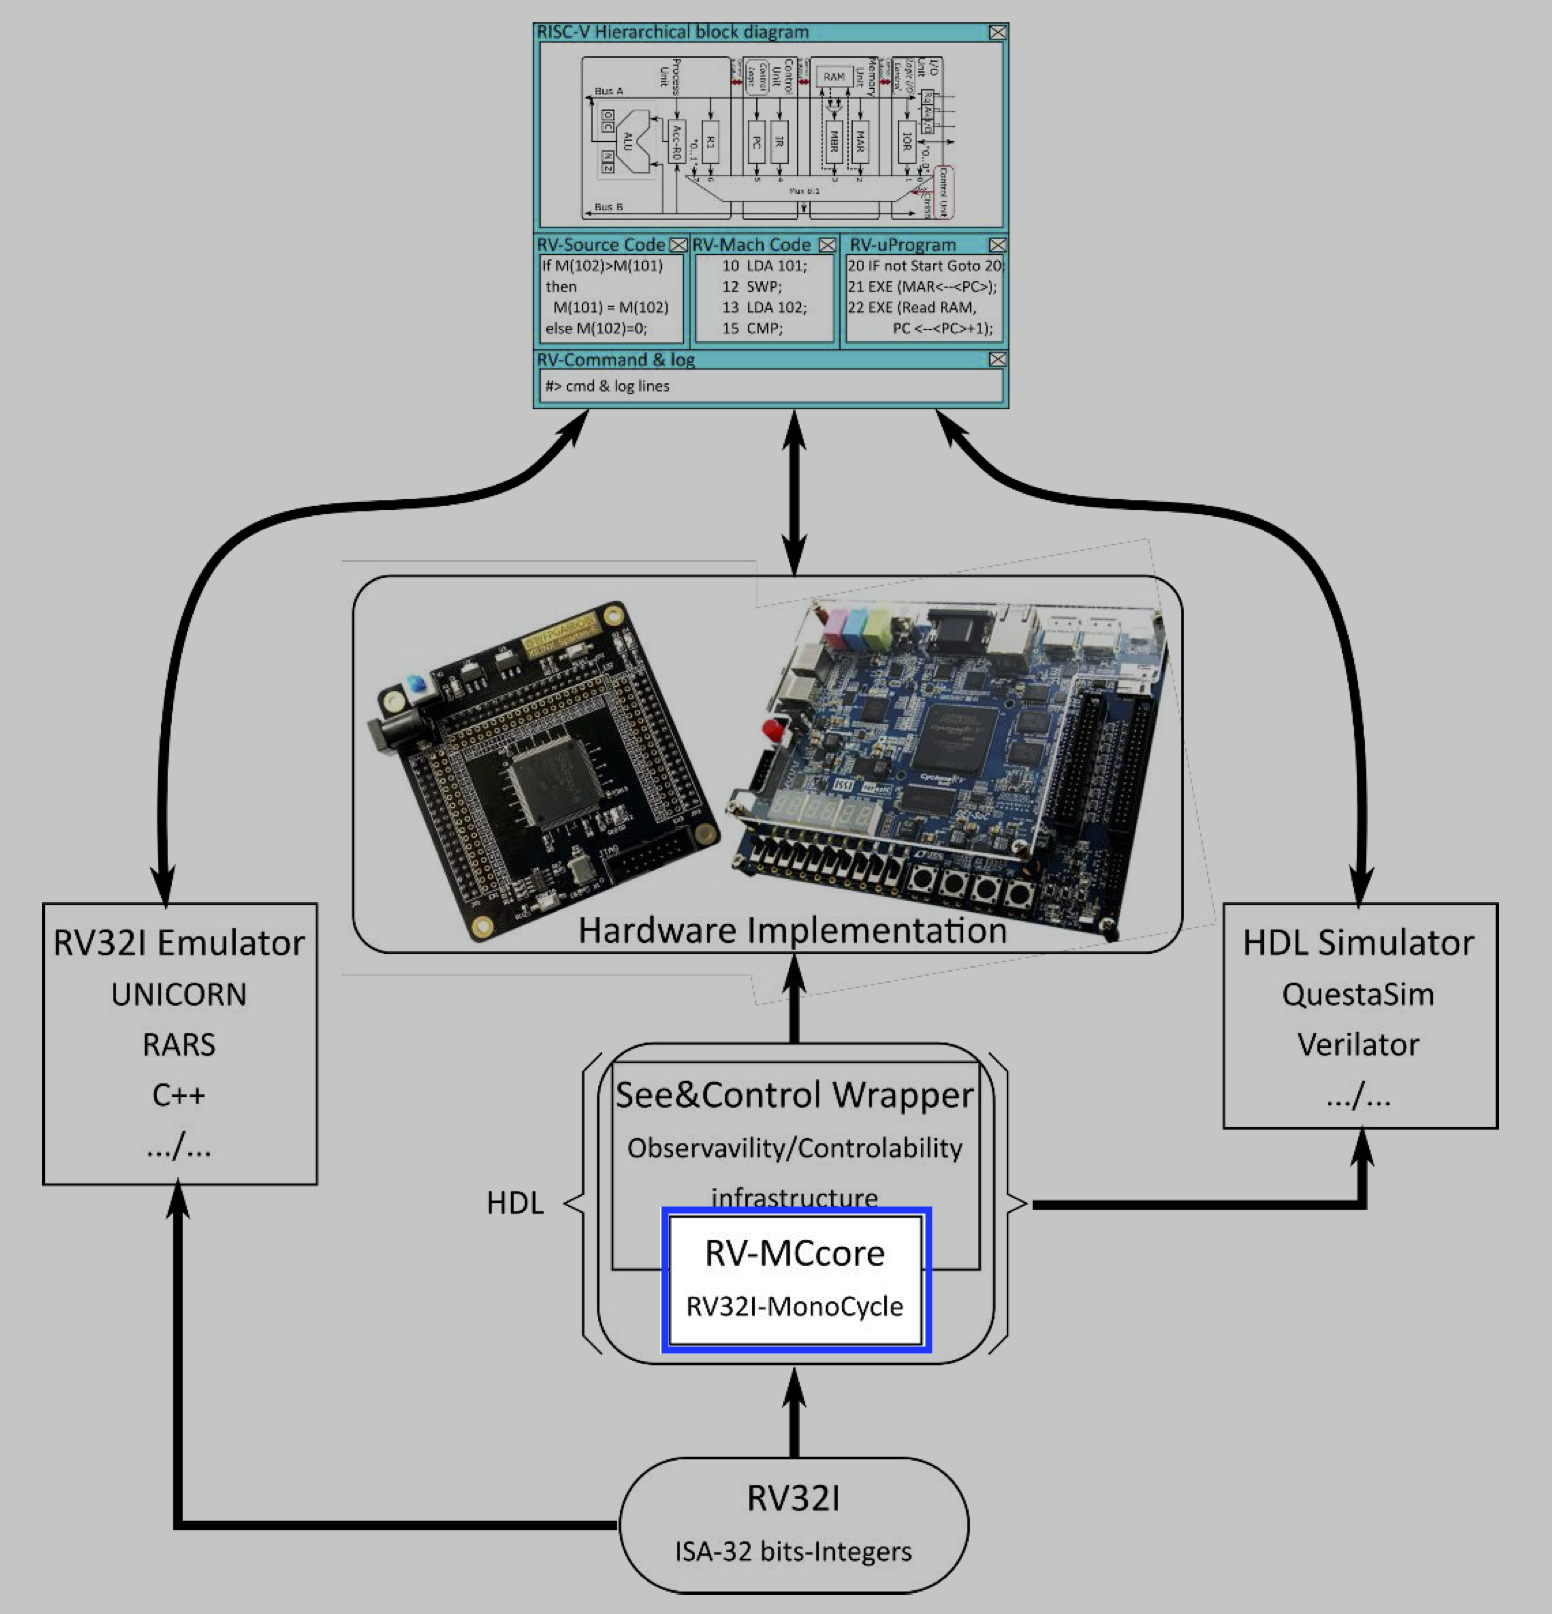
\includegraphics[width=\linewidth]{img/core_stack.png}
        \caption{Entron didàctic complert. Nucli marcat en blau per ubicar on s'engloba l'objectiu princiopal del treball}
        \label{fig:core_stack}
    \end{figure}

Aquest Treball Fi de Grau pretén proposar el disseny d'un nucli de processador RISC-V amb l’objectiu d’anar avançant cap un entorn didàctic per conèixer aquest tipus de processador. Des del propi nucli del processador, encerclat en blau a la figura \ref{fig:core_stack}, fins a un entorn gràfic que permeti mostrar l'execució de programes escrits en C, indicant quines parts del nucli es fan servir.
Tot això com a eina didàctica per entendre el funcionament dels computadors d'arquitectura RISC amb conjunt d'instrucció que està guanyant quota de mercat. 

Concretament, la micro-arquitectura que s'implementarà consistirà en un subconjunt del repertori d’instruccions, el \textbf{ISA-RV32I}, que es el que ha d'incloure cada processador basat en l'arquitectura RISC-V amb 32 registres. 
Aquest nucli serà mono-cicle i d’execució seqüencial d’instruccions. 

A la secció \ref{sec:Obj} es detallen els objectius, i seguidament es fa una visió a l'estat del art relacionat en l'entorn de RISC-V. A la secció \ref{sec:Core} S'entra en detall al disseny del propi nucli. A la secció \ref{sec:Pulp} es comenta un canvi de disseny per a poder utilitzar diferents tipus de memòries. L'apartat \ref{sec:Test} tracta del sistema utilitzat per provar el funcionament del disseny. Al següent apartat \ref{sec:FPGA} es tracta la implementació i física del processador. A les últimes seccions es mostra la metodologia seguida en aquest treball i una reflexió del projecte desenvolupat i de treball futur.



\section{Objectius} 
\label{sec:Obj}
El principal objectiu d'aquest treball és produir un disseny d'un nucli RISC-V de 32 bits a nivell RTL (Register-Transfer Level) en Verilog, on el codi sigui fàcil de seguir, implementar-lo en una FPGA (Field-Programmable Gate Array) i comprovar que és capaç d’executar programes compilats amb eines compatibles amb RISCV. El processador serà monocicle (s'executa una instrucció en cada cicle de rellotge), sense pipeline ni branch prediction.

Aquest objectiu es pot dividir en diferents subobjectius:

\begin{itemize}

    \item Aprendre a dissenyar un computador des de zero fent recerca d'informació. Aquesta recerca es basarà en consultar els documents de l’estàndard de l'ISA de RISC-V \cite{waterman_volume_2019} \cite{waterman_volume_2019-1}, així com altres llibres que es centren més en el disseny de nuclis de processadors \cite{patterson_computer_2018} o en el llenguatge de descripció de hardware utilitzat, en aquest cas Verilog \cite{li_implementing_2018}.

    \item Especificar i dissenyar a nivell HDL-RTL un nucli RISC-V amb el subconjunt bàsic d'instruccions de l’ISA, el RV32I, que permeti l'execució de programes simples escrits en C. El codi HDL ha de ser llegible i sintetitzable.
    
    \item Preparar un Testbench per a comprovar el funcionament del nucli.
    
    \item Descriure fluxes de desenvolupament utilitzant contenidors i altres coneixements del grau que facilitin el disseny i la validació del nucli RISC-V.  
    
    \item Materialitzar i testejar el nucli anterior en una placa de desenvolupament basada en FPGA.
    
        
\end{itemize}

\section{Estat del Art}
\label{sec:Art}
Actualment existeixen diversos dissenys de nuclis \footnote{\href{https://github.com/riscv/riscv-cores-list}{https://github.com/riscv/riscv-cores-list}} llistats a la ``RISC-V fundation'', organització que proporciona eines, suport i vetlla per al projecte RISC-V. Aquests nuclis implementen molts dels repertoris definits en l'ISA, alguns fins i tot el repertori que s'ha decidit implementar, el RV32I, i en el mateix llenguatge proposat ,Verilog. Aquests generalment afegeixen tècniques de ``pipeline'' (per accelerar el cicle de rellotge), interrupcions (per tenir subrutines que s'executin de manera asíncrona) o ``branch prediction'' (per reduir els cicles perduts a l'hora de fer salts de programa). 
Per aquest treball es vol generar un processador minimalista, sense aquestes funcionalitats, per tal de que sigui didàctic. 
El fet de no incloure blocs superficials fa que els alumnes puguin veure els blocs principals. 

Alguns d'aquests nuclis més coneguts són els Rocket i freedom de SiFive, una empresa que va sortir del grup de recerca que va dissenyar RISC-V. També existeix el RI5CY de l'Escola Federal Politècnica de Zuric (ETH Zurich), el nucli Ibex (antigament Zero-riscy) de l'organització lowRISC.
Cada un d'aquests nuclis tenen associada una llicència, algunes d'ús obert i altres no, i això és possible perquè la part oberta de RISC-V només és l'ISA, i per tant cada una de les implementacions pot introduir la llicència que cadascú vulgui, però normalment s'intenten crear projectes de Hardware obert que utilitzen llicències d'ús lliure.

Cal destacar que només amb el disseny dels nuclis no es té un computador complet, fa falta tot un entorn per a poder-se connectar amb memòries i perifèrics. 

Per obtenir el disseny d'un computador complet existeixen diferents projectes que proporcionen de mòduls externs al nucli per a poder connectar-se a un bus, a un port sèrie o controlar un conjunt de ports Entrada/Sortida per a un ús general. Alguns exemples d'aquestes plataformes són Rocket Chip de SiFive, PULPino de la ETH Zurich o LowRISC de lowRISC, on cada una d'aquestes disposa de diferents mòduls que acompanyen el nucli.

Amb aquests projectes es genera un SoC (Sistem on Chip) que pot ser implementat en una FPGA o en un ASIC (Application Specific Integrated Circuit).

En el cas d'aquest treball es vol dissenyar un nucli simple i senzill des de zero, que pugui ser portat a una de les plataformes anteriorment esmentades.
%\section{Finalitat del projecte}

\section{Core Risc-V}
\label{sec:Core}
    A l'hora de dissenyar la micro-arquitectura del processador és important analitzar bé el repertori d'instruccions per definir els elements que seran necessaris per poder executar les instruccions del repertori.
    
    L'ISA defineix el processador de tipus \textbf{Load/Store}, per tant no permet operar directament amb dades de memòria. 
    Sempre s'ha de llegir un valor, guardar-lo en un banc de registres i en una nova instrucció operar amb el registre.
    De manera semblant a l'hora de guardar un valor només es pot fer des d'un registre, per tant no es poden guardar directament resultats d'operacions a memòria.
    Per poder identificar cada línia de programa es necessita un registre anomenat\textbf{ Program Counter}.

En aquesta secció es descriu en detall cada part del nucli. 
    \subsection{Instruction set}
    Per dissenyar un nucli de processador primer s'ha de determinar quin repertori d'instruccions haurà d'executar, per aquest motiu a continuació es descriu com està composat el repertori RV32I, utilitzat per al disseny del nucli en qüestió.
        %\subsubsection{RV32I}
    S'ha escollit el repertori RV32I degut a que és el més bàsic de RISC-V, la base pels processadors RISC-V de 32 bits. Permet fer operacions aritmeticològiques amb nombres enters, llegir i guardar dades a memòria externa, així com salts condicionals i incondicionals dins un programa. A sobre d'aquest repertori es poden afegir extensions per a fer altres operacions com multiplicació i divisió, però queden fora d'aquest treball. 
        
    
    
    \begin{figure}[!h]
    \centering
    	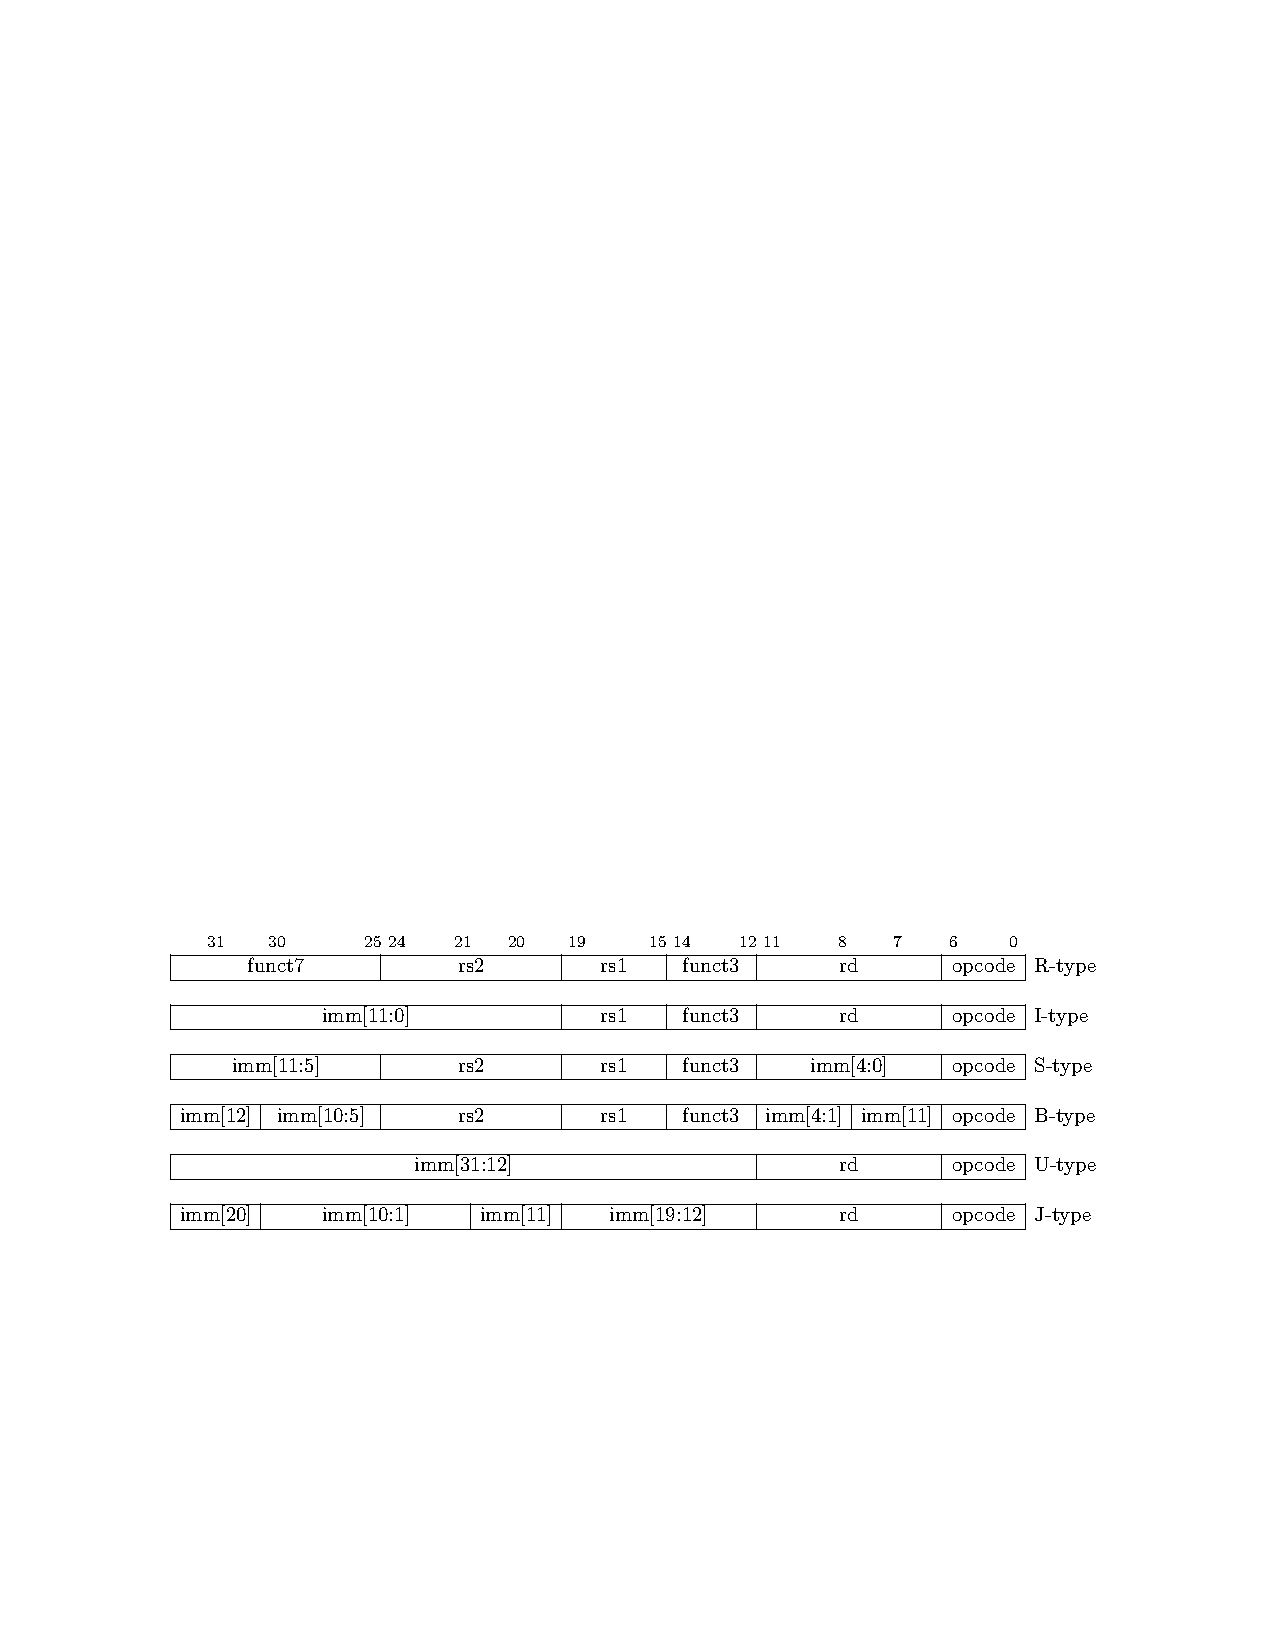
\includegraphics[width=\linewidth]{pdf/Encoding.pdf}
        \caption{Codificació del tipus instruccions del repertori RV32I.}
        \label{fig:baseinstformatsimm}
    \end{figure}
    
    Per a poder analitzar el conjunt d'instruccions s'ha decidit dividir-lo en quatre grups segons l'acció que s'efectua:
    
    \begin{itemize}
        \item Aritmeticològiques: operacions que utilitzen dos operands font d'un banc de registres, o un registre i un valor immediat provinent de la instrucció. Realitzar una operació aritmeticològica amb els operands, i guardar el resultat en un registre destí del banc de registres.
        \item Lectura o escriptura de dades a memòria externa: operacions per moure dades des de la memòria de dades al banc de registres i viceversa. A partir d'una posició adreçada per byte es guarda una dada de la memòria externa a un registre del banc de registres, o anàlogament guardar una dada d'un registre intern a una posició de memòria externa.
        \item Salts d'execució: operacions que permeten modificar el flux d’execució d’un programa, canviant l’adreça de la següent instrucció a llegir de la memòria de programa. Ja sigui després d'avaluar una comparació entre dos registres o de manera incondicional.
        \item Control del processador: operacions relacionades amb registres d'estat i de control del processador i sistema d'interrupcions. En aquesta implementació no hi ha cap interrupció i els registres de control implementats son els mínims per complir amb l'especificació de RV32I en mode usuari.
    \end{itemize}
    
    A l'hora de codificar les instruccions existeixen els tipus descrits a la figura \ref{fig:baseinstformatsimm}.
    
    Les instruccions aritmeticològiques poden obtenir els operands d'entrada des de valors guardats en registres (\textit{rs1} i\textit{ rs2}) amb instruccions de tipus \textbf{R}, o amb valors immediats incrustats a la instrucció (\textit{imm}), amb instruccions de tipus \textbf{I}. També hi ha trobar el cas d'instruccions que guarden un valor immediat (\textit{imm}) de 20 bits a un registre \textit{rd}, utilitzen el tipus \textbf{U}.
    
    Les instruccions de salt incondicional poden utilitzar els tipus \textbf{I} per definir el desplaçament com a la suma del valor que conté el registre \textit{rs1} i el valor immediat (\textit{imm}), o el tipus \textbf{J} per definir el desplaçament directament amb valor immediat (\textit{imm}).
    Per salt condicional s'utilitzen les instruccions de tipus \textbf{B}, indicant els registres a comparar (\textit{rs1} i \textit{rs2}) i el desplaçament amb el valor immediat (\textit{imm}).
    
    Les de lectura utilitzen el tipus \textbf{I}, aprofitant el valor del registre \textit{rs1} com a base, el valor immediat (\textit{imm}) com a desplaçament i \textit{rd} per identificar el registre on guardar les dades.
    Per l'escriptura de dades a memòria s'utilitza el tipus \textbf{S}, aprofitant el contingut del registre \textit{rs2} com a valor a guardar, \textit{rs1} com a l'adreça base i l'immediat (\textit{imm}) com a desplaçament a partir de la base.
        
    Les instruccions per accedir als registres de control i estat utilitzen la codificació de tipus \textbf{I}, utilitzen el valor immediat (\textit{imm}) com a adreça del registre d'estat o control, el valor del registre \textit{rs1} com a valor a modificar i el registre \textit{rd} com a destí per guardar el valor del registre d'estat o control.
    
    %\subsection{Arquitectura}
    
    Per poder executar aquestes instruccions es necessiten els següents blocs principals:
    \begin{itemize}
        \item Unitat de control: s'utilitza per configurar la resta d'unitats amb les dades i opcions pertinents per a arribar a executar la instrucció carregada de la memòria de programa.
        \item Comptador de programa, en anglès ``Program Counter'' (PC) i unitat de lògica de salt, en anglès ``Branching'' (BR): per mantenir l'adreça de la instrucció actual i poder-la utilitzar per a determinar el valor de la següent adreça de programa. L'adreça s'envia a la memòria de programa per a obtenir la següent instrucció i continuar amb l'execució, a una instrucció per cicle de rellotge.
        \item Banc de Registres: per mantenir dades provinents de valors definits a la pròpia instrucció (valors immediats) o llegits anteriorment de la memòria de dades. El nucli només podrà operar amb dos valors (\textit{rs1} i \textit{rs2}) corresponents a dos registres que es trobin dins el banc i/o amb valors immediats, per tant no pot operar directament amb paraules de memòria. El banc té 32 posicions de memòria de 32 bits cada posició. Està especificat per l’estàndard RISCV.
        \item Unitat aritmètica-lògica, en anglès ``Arithmetic Logic Unit'' (ALU): per executar les operacions aritmètico-lògiques dels programes amb dades del banc de registre i/o valors immediats.
        \item Unitat de Lectura-Escriptura, en anglès ``Load–Store Unit'' (LSU): per executar les instruccions de lectura i escriptura de la memòria de dades. Aquesta a més pot emmascarar les dades per a poder fer accessos a paraules senceres de memòria (32 bits), mitges paraules (16 bits) o a bytes (8 bits) i fer accessos desalineats.
        \item Unitat d'execució: engloba la ALU, BR i LSU i afegeix elements per decidir quines dades entren a cada unitat i quina de les unitats pot escriure  al banc de registres.
        \item Registres de control i d’estat, en anglès ``Control and Status Register'' (CSR): per les instruccions especials per a la modificació dels CSRs. Aquestes permeten extreure informació de rendiment del processador així com modificar-ne la seva configuració. En aquesta implementació només s'inclouran els registres d'estat que descriuen el rendiment.
    \end{itemize}
    



    \label{sec:arch}
    \begin{figure*}[!ht]
    \centering
    	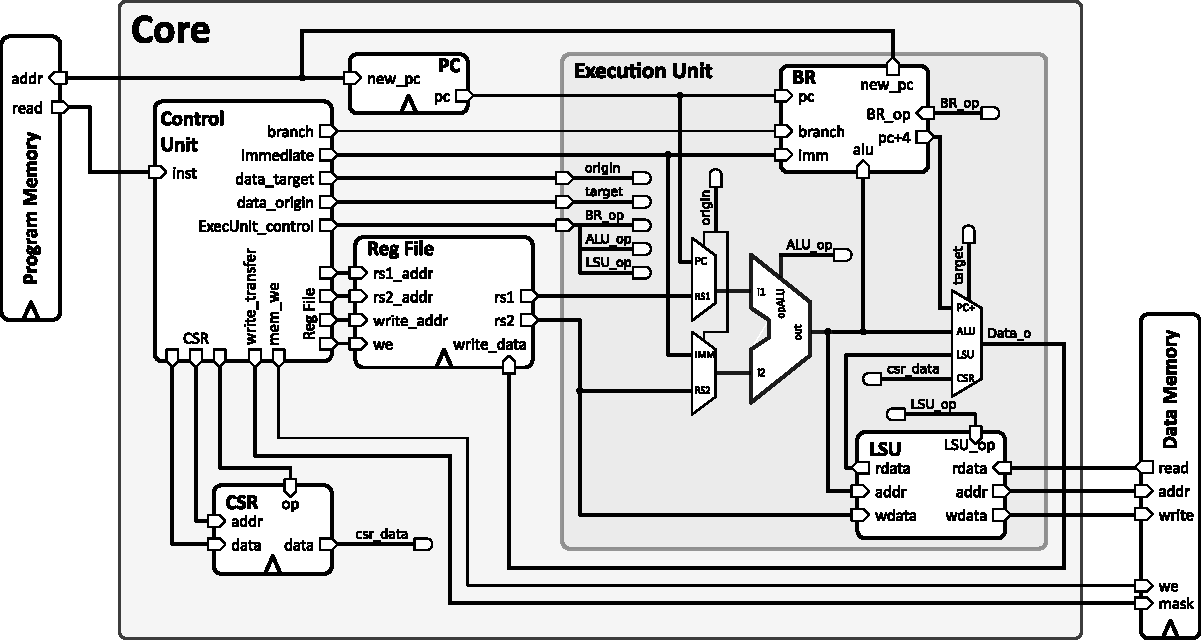
\includegraphics[width=0.9\linewidth]{pdf/arch_RiscV.pdf}
        \caption{Arquitectura del Nucli. Esquema de blocs de la distribució i connexions entre les diferents unitats i elements.}
        \label{fig:core_arch}
    \end{figure*}
    
    %A la figura \ref{fig:core_arch} es pot veure un esquema de blocs general que mostra les unitats principals. Aquestes es poden diferenciar en dos tipus: les que implementen únicament lògica combinacional i les que també implementen lògica seqüencial (aquests tenen elements de memòria i necessiten d'un senyal de rellotge i de reinici).

    
    La manera que estan interconnectats tots aquests mòduls es mostra al diagrama de blocs del processador de la figura \ref{fig:core_arch}. Aquests mòduls es poden classificar en dos blocs, els de lògica combinacional i els seqüencials. 
    
    En el primer grup s'inclou: la unitat de control, la unitat d'execució i dins d'aquesta les unitats de càlcul aritmeticològic, de salt de programa, càrrega i escriptura de dades a memòria. Aquestes unitats es limiten a fer operacions de transformació de instruccions a senyals de control i dades (unitat de control), operacions aritmeticològiques (ALU), de càlcul de la següent adreça de programa (BR) o d'emmascarament de dades a l'hora d'accedir a memòria (LSU) respectivament.
    
    En el segon grup (mòduls seqüencials) s'inclou el comptador de programa, banc de registres i la unitat de CSR.
    Aquestes unitats guarden dades que reben com a entrada o de comptadors interns en el cas de la unitat de CSR i les mantenen a la sortida fins al següent cicle de rellotge. 
    
    Com a exemple de com interactuen les unitats, podríem definir que, un cop la unitat de Branch (BR) genera l’adreça de la següent instrucció de programa a capturar a partir de l'adreça que actualment guarda el comptador de programa (PC). 
    Es càrrega una única instrucció per cicle de rellotge. Aquesta és descodificada per la unitat de control. 
    Per exemple, per les instruccions aritmeticològiques descodifica a partir de la instrucció obtinguda de memòria les adreces \textit{rs\_addr1} i \textit{rs\_addr2} dels operands font i l’adreça \textit{write\_addr} corresponents a registres concrets del banc de registres. 
    D’aquesta manera als dos busos \textit{rs1} i \textit{rs2} del banc de registres hi tenim els valors dels operands font que es passen a la ALU. La unitat de control també genera el codi d’operació \textit{ALU\_op}, que indica quina operació sobre els dos operands ha de fer la ALU. 
    La sortida d’aquesta es posa al bus \textit{write\_data} del banc de registres que té el senyal d’escriptura \textit{we} habilitat. 
    Per les instruccions amb immediats, el funcionament és molt semblant a l’anterior però el valor d’un dels operands fonts no es troba al banc de registres sinó a la part immediata de la instrucció. Per aquest motiu el valor immediat no pot ser de 32 bits, normalment és de 12 o 20 bits i s'estén el signe per a obtenir un valor de 32 bits i poder operar amb ell.

    
    D'una forma semblant les operacions de lectura o escriptura obtenen la instrucció de la mateixa manera, però a l'hora de generar els senyals de control, es defineix quin registre conté l'adreça base, així com el nombre de bytes que s'ha de desplaçar des d'aquella posició com a dada immediata. En cas de fer una lectura es necessari indicar a quin registre s'escriurà la dada i activar el senyal d'escriptura de registre com el cas anterior. S'utilitza la ALU per sumar l'adreça i el desplaçament per obtenir l'adreça final de la paraula de memòria a llegir o escriure. La unitat de control també determina la mida de les dades amb les que s'operarà (paraula sencera, mitja paraula o byte). La unitat LSU s'encarrega de comunicar-se amb la memòria i obtenir o escriure les dades. A través de les senyals \textit{addr} per indicar amb quina adreça de memòria treballar, \textit{rdata} per llegir el valor de la memòria i \textit{wdata} per escriure-hi, en aquest últim cas també s'activa el senyal \textit{mem\_we} per permetre l'escriptura. També s'activa el senyal \textit{write\_transfer} que indica amb una màscara de 4 bits quins bytes dels 4 que conformen una paraula s'estan modificant, prement els accessos desalineats.
    
    A l'hora de fer salts de programa s'utilitza la dada del PC com a base i avaluant amb la ALU si es tracta d'un salt incondicional sumar el valor immediat de la instrucció al PC, o a l'adreça guardada en un registre, i aquest utilitzar-lo per a carregar la següent instrucció guardant el valor al PC al següent cicle de rellotge. També és necessari en certes operacions desar el valor del PC actual incrementat 4 bytes per a saber la direcció a la que haurà de tornar l'execució desprès del salt en un registre del processador indicat per la pròpia instrucció.
    
    Per a executar instruccions CSR la unitat de control ha de configurar els senyals necessaris per a que la unitat de CSR llegeixi el valor d'algun dels seus comptadors i escriure'l a algun registre, o modificar algun registre de control aplicant una màscara o modificant el valor directament.
    
    A les següents seccions es descriuen en detall les parts de l'arquitectura.
    \subsection{Senyals de Control}
    En aquesta secció es descriuen quins senyals fan falta per operar el nucli i els busos i línies de connexió interns que intercomuniquen les diferents unitats.
        
        %\subsubsection{Connexions externes}
        Els senyals bàsics per a poder operar el nucli des de l'exterior són:
        \begin{itemize}
            \item Els senyals de rellotge i reinici: el senyal de rellotge és bàsic per a poder determinar la freqüència a la que funcionarà aquest, és a dir cada quan els circuits seqüencials actualitzen les dades. El senyal de reinici s’encarrega d’inicialitzar el valor dels registres a un valor predeterminat. És necessari per inicialitzar el processador. 
            \item Senyals relacionats amb les paraules de programa: conformats per un bus d'adreça (\textit{new\_PC} de 32 bits), que determina la posició en bytes de la següent línia de programa llegir, i un altre bus (de 32 bits) que proporciona els 4 bytes que conformen una paraula de programa (\textit{inst}).
            \item Senyals relacionats amb la memòria de dades: conformats per un bus d'adreça (de com a molt 32 bits) que determina la posició en bytes de la dada que volem llegir o escriure, per un bus de 4 bits que determina una màscara de quins bytes interessa modificar, i també per un senyal d'un bit per determinar si es vol escriure o llegir de la memòria i un altre bus (de 32 bits), que proporcionarà les dades que s'hagin d'escriure o llegir.
        \end{itemize}
        
        %\subsubsection{Senyals interns}
        A part de la distribució dels senyals de reinici i de rellotge a les unitats seqüencials existeixen dos principals grups de senyals: els referents a les dades que s'estan utilitzant i els referents al control de les operacions que fa cada unitat.
        
        En quant als referents a les dades es troben: valors immediats obtinguts de la instrucció base. En aquest grup s'inclou el valor ``immediate'' que surt directament de la unitat de control. %o el valor de csr\_data que surt de la mateixa unitat de control i arriba a la unitat de CSR
        També els senyals \textit{rs1} i \textit{rs2} sortints del banc de registres o els senyals \textit{rdata} i \textit{wdata} de la unitat LSU. Dins aquest grup s'afegeix també el senyal de PC degut a que pot ser utilitzat com a senyal d'entrada per a operacions. La propietat en comú que tenen tots aquests senyals es que son de 32 bits, definits per l'amplada de la paraula.
        
        En canvi pels senyals de control es troben diferents amplades de bus, per exemple els senyals referents a les adreces de l'accés a dades de memòria, així com els valors de \textit{rs1} i \textit{rs2} o de \textit{write\_addr} per a determinar quins registres ha d'utilitzar el banc de registres i el bus que determina l'adreça del registre CSR al qual es vol accedir. Per últim tenim la resta de senyals de control que determinen quin es el comportament de cada unitat. Tots aquests surten de la unitat de control i actuen sobre multiplexors com els senyals d'\textit{origin} i \textit{target} o busos que determinen quines operacions han d'executar cada un de les unitats com els senyals \textit{ALU\_op}, \textit{BR\_op}, \textit{LSU\_op} o \textit{CSR\_op}. En aquest últim grup s'inclouen també els senyals de \textit{write\_enable} que van tant al register file com a la memòria de dades.
        
        
    \subsection{Comptador de programa}
    
    El comptador de programa té la funció de mantenir el valor de l'adreça corresponent a la instrucció que s'està executant en un cicle de rellotge i poder utilitzar aquest valor per determinar a quina adreça següent demanar a la memòria de programa per a poder continuar l'execució.
    Degut a que aquest mòdul necessita guardar un valor és de tipus seqüencial, és a dir necessita d'un senyal de rellotge per a determinar quan ha de llegir noves dades i un senyal de reinici  per a modificar el seu estat a un de conegut, habitualment 0 per a començar l'execució d'un programa en aquesta adreça. 
    
    El PC consisteix bàsicament d'un registre que emmagatzema el valor de la següent adreça de programa, normalment generada per la unitat de Branching, a cada cicle de rellotge i mantenir el valor durant aquest període perquè altres unitats l'utilitzin per definir la següent adreça a demanar o guardar-ne el valor en un registre.
    
        \begin{figure}[!ht]
    \centering
    	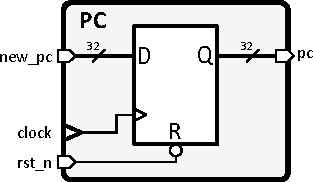
\includegraphics[width=0.5\linewidth]{pdf/PC.pdf}
        \caption{Representació del Comptador de Programa. Internament és un registre que carrega nous valors en el flanc de pujada del cicle de rellotge.}
        \label{fig:PC}
    \end{figure}
    La implementació d'aquest mòdul és molt senzilla, ja que consisteix en assignar una dada d'entrada a un senyal de sortida registrat a cada cicle de rellotge, o modificar el valor de dita sortida per 0 en el cas de detectar un senyal de reinici, com es veu a la figura \ref{fig:PC}. 
    
    
    \subsection{Unitat de Control}
        La unitat de control s'encarrega de descodificar la instrucció que rep com a entrada i generar els senyals necessaris per poder configurar la resta d'unitats internes del processador per dur a terme l'operació definida per la instrucció. Així com generar els valors immediats depenent del tipus d'instrucció.  
        
    \begin{figure}[!ht]
    \centering
    	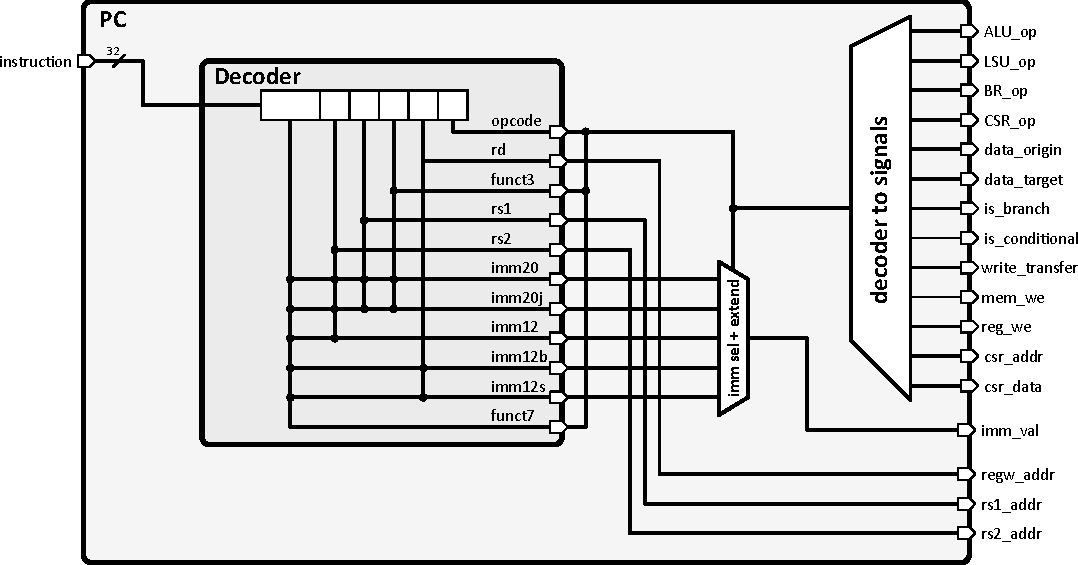
\includegraphics[width=\linewidth]{pdf/Control_Unit.pdf}
        \caption{Representació de la Unitat de Control. Esquema dels elements on es separa la instrucció en senyals interns i que després s'utilitzen per generar els senyals de control.}
        \label{fig:control}
    \end{figure}
    

    
    Per a dissenyar aquesta unitat, representada a la figura \ref{fig:control}, es defineix un mòdul amb un sol senyal d'entrada, que correspon a la instrucció provinent de la memòria de programa, i com a sortida tots els senyals de control. S'utilitzen paràmetres per definir l'amplada de les dades tant d'entrada com de sortida.
    El comportament d'aquesta unitat s'ha dissenyat en dos parts, una primera de descodificació que consisteix en definir senyals interns que seleccionen les diferents parts que conformen una instrucció del repertori, concretament en el codi d'operació que coincideix amb els 7 bits menys significatius, en les adreces dels registres interns (\textit{rs1}, \textit{rs2} i \textit{rd}), en els selectors de tipus d'operació (\textit{funct3} i \textit{funct7}) i en el valor immediat per a als diferents tipus d'operació.
    
    Un cop generats aquests senyals es defineix un altre descodificador, segons el codi d'operació i els senyals de tipus d'operació. On en cada combinació de codis es determinen els estats que tindran cada un dels senyals de control, com s'estendrà el valor immediat una dada de 32 bits si en té, i en el cas d'utilitzar un selector de tipus d'operació hi ha una altra directiva case que permet definir com configurar cada senyal de control per a cada cas concret.
    
    
    
    
    %*Destacar que consta de dos parts principals, una primera part que separa la paraula de programa en els blocs que defineix la especificació de RiscV i després un sistema que tria quines senyals de control activar segons els codis d'operació.
    
    \subsection{Banc de Registres}
    Per poder operar amb dades fa falta poder guardar-les, i per aconseguir aquesta funcionalitat s'utilitza un banc de 32 registres de 32 bits que permet guardar una dada a un registre a cada cicle de rellotge, el que permet obtenir dues dades diferents del banc a la vegada identificades per adreces.
    Degut a que aquest mòdul ha d'emmagatzemar dades també és de tipus seqüencial, és a dir, necessita un senyal de rellotge i un de reinici per esborrar les dades existents i determinar el valor de cada registre intern.
    
    \begin{figure}[!ht]
    \centering
    	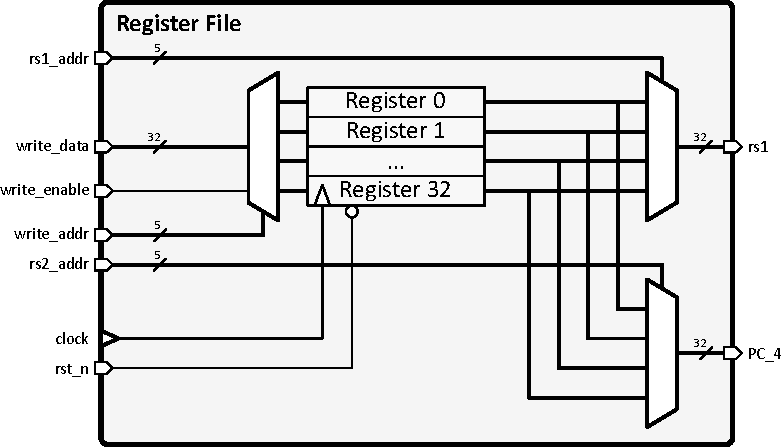
\includegraphics[width=0.9\linewidth]{pdf/regfile.pdf}
        \caption{Representació del Banc de Registres. Esquema dels elements interns, es pot veure el banc i els multiplexors per seleccionar quins senyals posar a la sortida o escriure als registres.}
        \label{fig:regfile}
    \end{figure}
    
    Aquest mòdul s'implementa d'una manera semblant al comptador de programa, però degut a que en aquest cas existeix més d'un sol registre i existeixen dues sortides és necessari afegir busos d'entrada que determinin tant les adreces de cada un dels registres que es voldran llegir a la sortida així com l'adreça del registre al qual es vol escriure. També és necessari dotar a aquest mòdul d'un senyal que permeti decidir quan llegir noves dades al registre escollit per escriure, ja que no totes les operacions necessiten escriure dades al banc de registres. Una representació d'aquesta implementació es pot veure a la figura \ref{fig:regfile}.
    
    
    
    
    \subsection{Unitat d'execució}
    Per compartimentar millor el nucli, s'ha definit un bloc d'execució que engloba les unitats de càlcul aritmeticològic, d'accés a memòria, i de salts de programa.
    
    Aquesta unitat s'encarrega de seleccionar les dades d'entrada que necessiten cada una de les subunitats segons els senyals provinents de la unitat de control, així com de decidir quina sortida de les diferents subunitats o de la unitat de CSR retorna al banc de registres, com es pot veure a la figura \ref{fig:core_arch}.
    
    Per determinar quines dades entren a la unitat aritmeticològica, la unitat de control genera un senyal de 2 bits (\textit{origin}) que determina, amb l'ús de multiplexors, si al primer port \textit{i1} de la ALU entra el valor del registre \textit{rs1} o el valor del PC per a calcular salts. De manera similar es determina en el segon port (\textit{i2}) si les dades que s'utilitzaran serà el registre rs2 o el valor immediat.
    
    D'una manera similar a la anterior es defineix un multiplexor, controlat pel senyal \textit{target} que permet triar entre les sortides de les tres sub-unitats o de la unitat de CSR quina d'aquestes dades serà retornada al banc de registres.
    
    La implementació d'aquest mòdul consisteix en declarar els submòduls de Branch, ALU, LSU, generar les connexions necessàries per a connectar els senyals de control provinents de la unitat de control i afegir els multiplexors que defineixen les entrades com es veu a la figura \ref{fig:core_arch}. 

    

    
    
    \subsection{Unitat Aritmetico-Lògica}
    Per poder operar amb les dades que ja tenim carregades al banc de registres fa falta una unitat aritmeticològica que serà la que efectuarà les operacions combinacionals per obtenir la funcionalitat esperada segons el tipus d'operació indicat, com per exemple  les operacions de suma, resta, desplaçament, comparació, XOR, OR o AND.
    
    Degut a que aquest element és conegut es representa la seva implementació com un mòdul específic ALU, com el del centre de la figura \ref{fig:core_arch}.

    
    \subsection{Unitat de Lectura i escriptura (LSU)}
    
    Per accedir a la memòria de dades utilitza la unitat de Lectura i escriptura (LSU), que s'encarrega d'aplicar una màscara a les dades segons el tipus d'accés: paraula sencera (32 bits, 4 bytes), mitja paraula (16 bits, 2 bytes), byte (8 bits, 1 byte). També és la unitat que connecta amb la memòria externa a través dels senyals \textit{addr}, \textit{rdata} i \textit{wdata}, per identificar l'adreça d'accés, les dades llegides i per escriure respectivament.
    
    Per implementar aquest mòdul fa falta que a partir dels senyals de control generats per la unitat de control es determini quins valors del 32 que van o tornen de memòria es deixen com estan i quins es posen a zero.
    
    \subsection{ Càrrega d'instruccions i unitat de salts (Branch)}%Fetch and Jumps}
        Per l'execució d'un programa el nucli ha de proporcionar a la memòria de programa quina adreça necessita perquè la resta del nucli la pugui processar al següent cicle de rellotge. Aquesta funcionalitat la proporciona la unitat de salts. 
    
    \begin{figure}[!ht]
    \centering
    	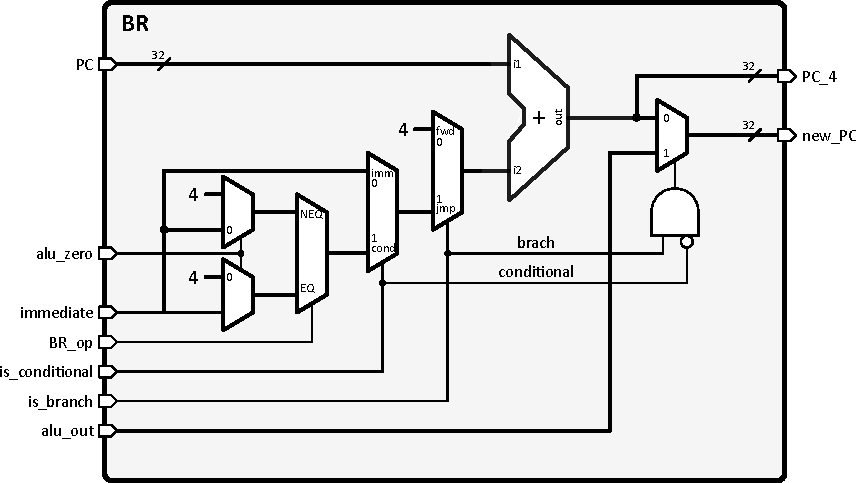
\includegraphics[width=\linewidth]{pdf/Branch.pdf}
        \caption{Representació de la Unitat de Salts. Esquema intern on es mostra el selector per a decidir l'increment del PC, de forma habitual aquest serà de 4 i segons la operació de salt agafarà altres valors.}
        \label{fig:BR}
    \end{figure}
    
    De manera normal, la funció bàsica d'aquesta unitat serà la d'incrementar el valor del PC actual en 4 per avançar els 4 bytes (32 bits) que ocupen les instruccions de programa, per poder processar el codi en ordre i de manera seqüencial. Ara bé, quan s'executa una operació de salt, aquesta unitat ha d'ésser capaç de en lloc de sumar 4 al PC actual, haurà de sumar el valor que vingui determinat per la instrucció de salt concreta (valor immediat o desat en un registre) de manera incondicional o sempre que es compleixi certa condició. Es pot saber si la condició es compleix si el valor de sortida de la ALU és 0 o no. Es pot veure com es representa aquesta funcionalitat en el diagrama de la figura \ref{fig:BR}.
    
    Per implementar aquesta unitat en Verilog és necessari generar el senyal de PC més 4 per una banda per poder ser guardat en un registre o carregat al PC, o sumar el valor del PC a un valor immediat i llegir-lo al comptador de programa. Es duu a terme seleccionant la operació convenient amb els senyals de la unitat de control, que determinen si es tracta d'una operació de salt incondicional o de salt condicional, i en aquest cas quin tipus d'operació s'està avaluant per a determinar si saltar o no depenent si la ALU té un zero a la sortida o no.
    
    
    \subsection{CSR}
    La unitat de Control and Stattus Register consisteix en tenir a disposició diferents comptadors que donen informació del rendiment del processador o que permeten determinar estats del mateix. 
    En aquest cas degut a que s'ha decidit implementar el conjunt més simple en mode usuari, el conjunt de CSRs és molt reduït, en concret només tres: 
    \begin{itemize}
        \item CYCLE: s'encarrega de comptar el nombre de cicles executats d'es d'un moment en el temps.
        \item TIME: aquest és un "real-time clock" a partir d'una freqüència determinada, en aquest cas serà la mateixa que la del rellotge del sistema.
        \item INSTRET: s'encarrega de comptar el nombre d'instruccions retirades o executades.
    \end{itemize}
    
    Degut a que en aquest cas es tracta d'un processador d'un sol cicle i amb un sol fil d'execució, el valor d'aquests 3 registres serà el mateix. Per facilitar la implementació s'ha decidit utilitzar un sol comptador.
    
    Per poder accedir a aquests registres, s'utilitzen unes instruccions concretes que indiquen el tipus d'accés a les dades. Aquestes es poden modificar directament o mitjançant una màscara per a modificar certs bits del registre.
    
    A l'hora de programar aquesta unitat en Verilog, s'ha fet una descripció no òptima degut a la falta de temps.
    

    
    \subsection{Processador RISC-V complet}
    
    Amb les unitats descrites anteriorment es pot muntar el disseny del nucli complet. Creant un mòdul anomenat Core, incloent les unitats especificades anteriorment i generant els senyals necessaris per a interconnectar-les com es veu a la figura \ref{fig:core_arch}.
    
    Degut a que en aquest cas el disseny és bastant simplificat l'execució es fa sense pipeline, és a dir, en un sol cicle de rellotge s'executa la instrucció indiferentment del tipus, i per tant s'han hagut de fer certes consideracions a l'hora de definir les memòries. 
    Amb aquest plantejament, com que en un sol cicle s’ha d’executar la instrucció sencera, és necessari que al demanar l’adreça de la dada que es vol llegir, la dada ha d’estar disponible abans del primer cicle de rellotge. 
    
    Les memòries reals no funcionen d'aquesta manera, normalment al demanar una adreça aquesta queda registrada dins el mòdul de memòria i al següent cicle de rellotge es quan la dada està disponible. Per aquest motiu les memòries del model inicialment proposat s'han implementat com a bancs de registres. Tenen un funcionament asíncron al proporcionar l'adreça, s'obté el valor de la dada de manera immediata. En una secció posterior s'explora una solució per poder treballar amb memòries síncrones implementades amb SRAM (Static Random Access Memory) on les dades estan disponibles un cicle de rellotge després.
    
    Per implementar les memòries es pot basar en el model del banc de registres, però en aquest cas nomes tindrà una entrada i una sortida.

        
        
\section{Core Risc-V adaptat a memòries síncrones}
\label{sec:Pulp}
    Degut a que per les decisions preses a l'apartat anterior no es pot utilitzar el nucli en un entorn amb memòries síncrones, és necessari complicar lleugerament el disseny per a adaptar-lo a entorns reals. 
    
    \begin{figure}[!ht]
    \centering
    	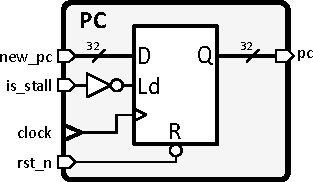
\includegraphics[width=0.5\linewidth]{pdf/PC_stall.pdf}
        \caption{Representació del PC adaptat al senyal de parada. Només s'afegeix un senyal que determina si el registre ha de guardar valors nous.}
        \label{fig:pc_stall}
    \end{figure}
    
    La primera observació va ser la necessitat de poder aturar l'execució del nucli per esperar a obtenir les dades disponibles, perdent rendiment de forma clara. La solució a aquest problema va ser afegir un senyal interna de parada, que evita que el PC carregui l'adreça de la següent instrucció, com es veu a la figura \ref{fig:pc_stall}. Això provoca que encara que el rellotge avanci el processador executa la mateixa instrucció una vega i una altra.
    
    Com es necessari modificar el nucli, i degut a que aquest està pensat per poder ser part d'un conjunt que necessitarà compartir recursos externs amb altres elements, s'ha decidit utilitzar una de les plataformes que permetin intercanviar el nucli de risc-v, proporcioni l'accés a la memòria i a un bus per a interconnectar altres elements.
    
    La plataforma que al final s'ha decidit utilitzar és PULPino \ref{cite pulp}. Aquesta proporciona un disseny de SoC que inclou diferents perifèrics com un GPIO, I2C (bus sèrie), UART (Universal Asynchronous Receiver-Transmitter) o SPI (Serial Peripheral Interface) entre altres, connectats a través d'un bus AXI4 (Advanced eXtensible Interface) (veure apèndix \ref{app:PULParch}). Això implica que l'accés a memòria és compartit amb la resta de perifèrics i pot ocórrer que el nucli i un perifèric vulguin accedir a la vegada i el nucli hagi de parar l'execució fins a no tenir disponible el recurs. Per controlar aquestes situacions s'utilitzen sistemes d'arbitratge. PULPino utilitza un protocol de ``request/acknowledge'', on el primer que demana l’accés el té concedit. Per demanar, accés (request), i la concessió amb un grant (acknowledge) (veure apèndix \ref{app:PULPtime}). 
    
    S'ha extret l'element que arbitra l'accés a les memòries de la plataforma i s'ha interposat entre el nucli i les memòries. Aquesta addició comporta senyals de control extres per a poder adaptar el nucli.
    
    Amb la possibilitat d'aturar l'execució del nucli l'adaptació a aquesta plataforma és factible.
    
    A continuació es mostren les modificacions necessàries per a adaptar el core a la plataforma PULPino:
    \begin{itemize}
        \item Nous senyals: senyals externs per demanar accés (\textit{request}) al bus de dades o de programa, així com senyals que garanteixen l'accés (\textit{grant}) i verificacions d'escriptura(\textit{rvalid}) segons el protocol proposat. El nucli realitza una sol·licitud per realitzar operacions de càrrega o escriptura a la memòria de dades, i queda bloquejat fins que es concedeixi l’accés.
        \item Estats: degut a que es necessari un protocol, es defineixen uns estats, i el nucli els ha de reconèixer i actuar de forma adient en cada un d'ells. 
        \item Parada del nucli: necessitat de parar l'execució del programa per esperar noves dades mentre el bus està ocupat per una altre recurs.

    \end{itemize}
    
    Per tant per adaptar el nucli és necessari generar uns senyals de request tant per la memòria de dades com per la de programa, que s'activarà cada cop que es vulgui accedir a memòria. El nucli quedarà a la espera del senyal que garanteix l'accés, i després esperarà mínim un cicle per a llegir les dades. En el cas de guardar dades a la memòria  intentarà escriure les dades fins que no rebi el senyal de validació de la transacció.
    Al haver de guardar un estat, i que depenent de senyals externs s’hagin de fer diferents operacions, serà necessària l’addició de diferents elements de memòria pel senyal de sol·licitud, i pel cas de la lectura caldrà una senyal (\textit{wait\_load}) que permeti esperar un cicle per fer la càrrega de la mateixa. 

    
        
        


\section{Desenvolupament i test}
\label{sec:Test}
% Una secció on es presenti el mètode d’avaluació dels resultats, els resultats en si mateixos, i una discussió/reflexió sobre aquests resultats.

Per provar el funcionament correcte del disseny s'han generat diferents tipus de proves.
A nivell de simulació en Verilog consisteixen en generar paraules de programa, carregar-les a l'array intern de la memòria de programa. Reiniciar el nucli i generar un senyal de rellotge durant cert nombre de cicles. Després analitzar l'estat d'algun registre intern o del PC i comparar-lo amb uns valors esperats. Aquesta aproximació permet generar proves pròpies per a cada una de les instruccions del ISA. Si en fer alguna modificació al disseny del nucli algun test falla es pot saber quin tipus d'operació és, i per tant identificar ràpidament l'error.

Un exemple d'aquest tipus de Testbench es preparar un petit programa que desi dos valors en dos registres interns, els sumi entre ells, el resultat es guardi en un tercer registre i al acabar l'execució verificar que a cert registre hi ha la suma dels dos primers valors. Per poder generar les paraules del programa es poden utilitzar Tasks de Verilog que generin els 32 bits segons l'especificació, per així parametritzar els elements de la instrucció i d'aquesta forma poder usar altres tipus de test (com per exemple sumar un valor positiu i un valor negatiu per verificar que les sumes amb signe funcionen). 



\section{Del RTL a la FPGA}  % Correu1.1
\label{sec:FPGA}
Un cop generat el codi RLT escrit en Verilog s’ha procedit a la implementació en una FPGA de la casa Intel en una placa de desenvolupament DE0 de TerAsic, aquesta proporciona elements com botons, interruptors, LEDs i pantalles de 7 segments. Per fer això ha estat necessari l'ús d'una eina de síntesi. En aquest cas s’ha utilitzat l'eina Quartus II d'Intel, per a verificar que el codi es sintetitzable. S’ha fet una primera síntesi per veure que el codi és completament comprensible per l’eina de síntesi, és a dir, que és capaç d’inferir el hardware descrit tal com es desitja. 
Un cop feta la síntesi, s'ha de dissenyar un entorn on el nucli pugui mostrar el seu funcionament amb món físic.
    \subsection{Embolcall FPGA}
        \begin{figure}[!ht]
    \centering
    	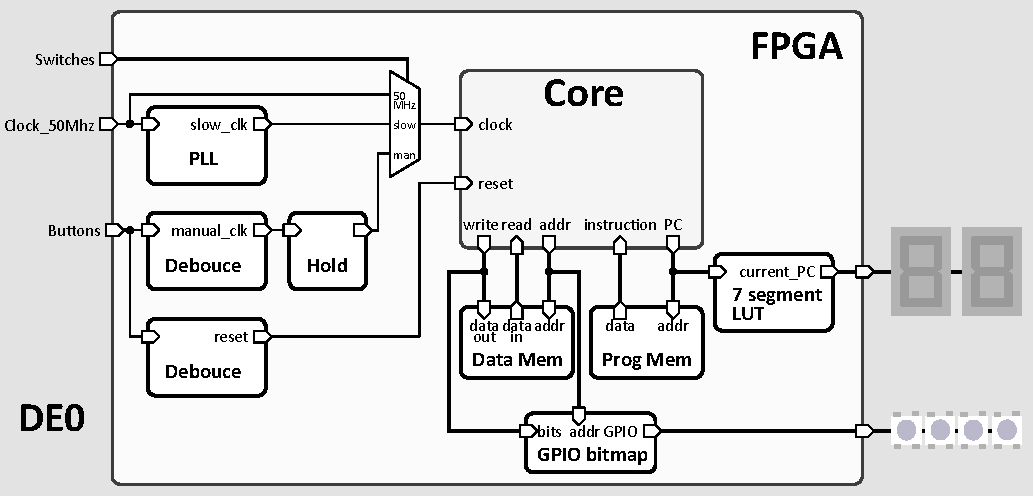
\includegraphics[width=0.9\linewidth]{pdf/arch_FPGA.pdf}
        \caption{Arquitectura de la FPGA. Esquema de blocs de la distribució i connexions entre les diferents elements.}
        \label{fig:FPGA_arch}
    \end{figure}
    
    El nucli per si sol no pot manifestar el seu funcionament més enllà de la modificació de dades de memòria. Per aquest motiu es necessari afegir una sèrie de components addicionals al processador per tal d’interactuar amb el mon extern, tals com mòduls que puguin eliminar el rebot a l'hora d'accionar un botó i poder utilitzar-lo coma senyal de reinici o rellotge. Un altre mòdul per interactuar amb el món físic és un
    descodificador que transforma dades de busos als senyals necessaris per a controlar pantalles 7 segments, aquest es pot utilitzar per mostrar el valor del PC. Per últim, un mòdul GPIO (General Purpose Input/Output) que controla senyals segons els valors d'una posició de la memòria de dades que permeten, per exemple, controlar LEDs. A part d'aquests mòduls, s'hauria d'incloure el mòdul del propi nucli i memòries com es veu a la figura \ref{fig:FPGA_arch}.

    
    \subsection{Programació FPGA}
    El disseny del processador no inclou una interfície per accedir externament a la memòria de programa, de manera que és necessari generar un fitxer d'iniciació de memòria. Aquest fitxer és carregat per una rutina inclosa en el codi Verilog, i per l’eina de síntesis per inicialitzar la memòria de programa que es tractada com una ROM (Read Only Memory). Un cop es sintetitza tot el mòdul es carrega el fitxer de bitstream a la FPGA i es fa un reinici del processador, les instruccions es comencen a executar. 
    
    \subsection{Funcionament}
    
    Per poder saber si el funcionament és correcte cal escriure un programa amb un estat final conegut i començar l'execució fins arribar a dit estat.
    Ara bé, s’ha introduït la possibilitat de fer córrer el processador molt a poc a poc, amb l'ús de mòduls PLL (Phase-Locked Loop), o directament generar un senyal de rellotge de manera manual, per poder veure l’execució de cada instrucció per qüestions didàctiques.
    
    Per verificar la lectura i escriptura de dades a memòria s'ha escrit un programa que escrigui valors a memòria, i aquests siguin utilitzats per a definir els valors de la paraula que està assignada al port GPIO per veure si els LEDs s'encenen de la forma esperada.
    
    A l'hora de provar el funcionament en FPGA s'han provat abans els tests en simulació de les seccions anteriors.
    Per a provar la FPGA s'ha escrit un programa que executi un bucle (operacions de salt) incrementant un valor (registres + ALU), i el carregui i guardi a la posició de memòria on la unitat de GPIO està implementada, i així poder veure físicament si el funcionament d'aquestes operacions funcionen en la implementació en FPGA. 



\section{Metodologia}
\label{sec:Method}
Primerament s'ha realitzat una part important de recerca sobre la ISA de RISC-V, amb alguns exemples d'implementació tant teòrics com funcionals. 
Un cop feta aquesta recerca s'ha procedit a proposar diferents dissenys, sobre el paper, de l'arquitectura a alt nivell amb unitats definides molt a nivell de funcionament. 
Després d'acordar un disseny general amb els tutors i la resta de l'equip, ha començat un procés de descripció en verilog del nucli, primer a alt nivell, determinant els blocs principals i certs senyals de control imposats per la ISA (com ara el codi d'operació). 
Un cop disposada aquesta versió inicial, s'ha procedit a un procés iteratiu de modificació d'aquest dissenys, afegint la funcionalitat per a les diferents instruccions del conjunt. En paral·lel s'han anat dissenyant els tests per a comprovar que les noves instruccions implementades funcionaven de manera correcta. 
Aquest procés ha sigut el més llarg degut a que a l'hora d'afegir noves instruccions han succeït diferents problemes. Aquests son deguts a decisions de disseny (com l'amplada de diferents senyals de control) o la ubicació de les funcionalitats dins de les pròpies unitats. 
Aquestes decisions de disseny s’han anat consensuant amb reunions amb  l'equip. 
Una vegada el disseny ha estat implementat per a tot el repertori d'instruccions, s'ha començat a preparar la implementació en FPGA i l'adaptació a les memòries síncrones. A la part final del projecte s'han fet els tests en FPGA que asseguren que el disseny funciona tant en simulació com en un entorn real.


\subsection{Flux de disseny}  % Correu1.2
Per desenvolupar la metodologia anteriorment explicada s'ha intentat utilitzar software obert (excepte la implementació en FPGA degut a que la proporcionada només funciona amb software propietari) i aplicar tecnologies de gestió i automatització per a facilitar la detecció d'errors. 

Per a l'edició del codi Verilog s'ha utilitzat l'editor de text \textbf{Visual Studio Code} (VSC) degut a que és de codi obert i permet afegir extensions que són de gran ajuda a l'hora de poder desenvolupar el projecte, en concret s'ha utilitzat una extensió anomenada ``\textbf{Verilog HDL/SystemVerilog}'' que permet executar una aplicació de \textbf{linting} (anàlisi d'errors en el codi) en temps real, fet que ajuda molt a no haver de guardar el codi i executar-lo externament i analitzar la sortida del compilador per a detectar errors. Com a compilador de verilog s'ha utilitzat \textbf{Icarus Verilog} degut a que es un programa opensource que permet executar testbench des de la línia de comandes. Per a executar els tests s'ha fet un petit script en \textbf{bash} per a llançar-lo com a tasca de compilació des de VSC. Per poder verificar que els senyals interns són correctes s'ha fet un buidat dels senyals en un arxiu .vcd i s'ha obert amb l'aplicació \textbf{Scansion} que és un visualitzador d'ones opensource.

A l'hora de gestionar el codi del propi nucli s'ha utilitzat \textbf{git} \footnote{\href{https://github.com/4a1c0/RV32i-Verilog}{https://github.com/4a1c0/RV32i-Verilog}} per poder tenir un històric del desenvolupament i informació de les modificacions que s'anaven fent al projecte. Per a assegurar-se que el disseny passa els tests i automatitzar-ne el procés s'ha utilitzat \textbf{docker}, \textbf{Icarus Verilog} i \textbf{Travis} per a poder generar un contenidor capaç d'executar els tests (docker + icarus verilog) i l'automatització amb Travis ja que proporciona el còmput i integració amb github que permet que amb cada modificació s'aixequi la imatge de docker abans creada i verifiqui el funcionament informant en cada commit. 

Aquesta primera part està basada en el disseny i test a nivell de simulació. A l'hora de fer síntesi el procés es basa inicialment de la mateixa manera, importar els documents Verilog del nucli però en l'aplicació \textbf{Quartus II} d'Altera. En aquesta aplicació s'ha desenvolupat l'entorn per a que el nucli pugui interaccionar amb la placa de desenvolupament \textbf{DE0} de TerAsic guardant els canvis en el mateix repositori de github.

Per a generar els codis de programa per als tests de la FPGA s'ha utilitzat el \textbf{riscv-gnu-toolchain} dins una imatge de Docker (per a no haver de tornar a compilar tot l'entorn cada cop) per a partir d'un codi en C poder compilar-lo amb \textbf{GCC} al repertori RV32I i poder posar el codi resultant com a inicialització de la memòria de programa de la FPGA.

\section{Conclusions i treball de futur}  % Correu1.3
\label{sec:conclusion}

Els objectius inicials s'han assolit correctament degut a que s'ha entregat un disseny de nucli RISC-V que implementa la extensió RV32I, el disseny està provat a nivell de simulació i a nivell físic amb la implementació de la FPGA. També s'han utilitzat eines que s'han après al llarg del grau per facilitar del manteniment de codi i/o la facilitat de poder utilitzar codi en contenidors i sistemes d'integració contínua per rebre avisos si no es passen correctament els tests.

A nivell de coneixements s'ha entrat en detall sobre com funciona un processador amb joc d'instruccions RISC i s'han dut a la pràctica els coneixements teòrics de les assignatures d'arquitectura de computadors.
Sobretot el principi de ``learning by doing'' fa que s'entenguin els conceptes en profunditat ja que es pot veure com implementar un concepte a mitges pot provocar un funcionament no esperat, com es el cas amb les memòries.

Com a treball futur es pot revisar i optimitzar el disseny del propi processador, sobretot simplificar la unitat de CSR ja que no es massa òptim, ja que que es una unitat que pot ser fàcilment extensible amb comptadors extres és millor utilitzar codi més simple.

També es poden millorar les prestacions del propi processador afegint pipeline per poder reduir el temps de propagació lògica combinacional de registre a registre i poder augmentar la freqüència del rellotge, així com per poder estar processant diferents etapes d'instruccions a l'hora i així augmentar el rendiment o throughput.

Degut a que aquest nucli es vol utilitzar per un projecte que permeti veure l'estat del processador en tot moment i poder modificar-ne l'estat del mateix, dissenyar un entorn de debug al voltant del nucli és un pas evident per a aconseguir aquesta funcionalitat.
    
    



\section*{Agraïments}

Agrair a en Raimon per proposar el treball sobre RISC-V i la gran feina de tutoria, al departament de microelectrònica, en concret a en Lluís, per poder adaptar el treball al entorn didàctic i el gran suport com a tutor. Als membres de la Red RiscV Ricardo i David per les propostes i correccions a les reunions de seguiment.
També agrair a la meva família pel suport durant el projecte, sobretot a la meva parella per ajudar-me a revisar informes. 
I com no a l'escola d'enginyeria i als companys d'estudis pels recursos i suport per arribar a realitzar aquest TFG. 


\bibliographystyle{IEEEtran}
\bibliography{references.bib}

%\begin{thebibliography}{11}
%\bibitem{latex}
%http://en.wikibooks.org/wiki/LaTeX

%\bibitem{2}
%Referència 2

%\bibitem{3}
%Etc.


%\end{thebibliography}
\newpage

\appendix

\section*{Apèndix}

\setcounter{section}{1}

    \subsection{Diagrama de temps del protocol per accedir a les memòries de la plataforma PULPino}
    \label{app:PULPtime}
    \begin{figure}[!ht]
    \centering
    	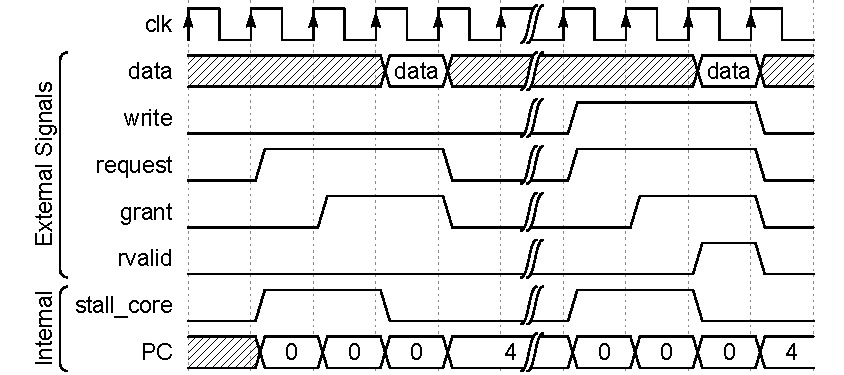
\includegraphics[width=\linewidth]{pdf/Stall_PC.pdf}
        \caption{Diagrama de temps de l'accés a memòria.}
        \label{fig:PULP_Temp}
    \end{figure}
    
        \subsection{Arquitectura de la plataforma PULPino}
        \label{app:PULParch}
    \begin{figure}[!ht]
    \centering
    	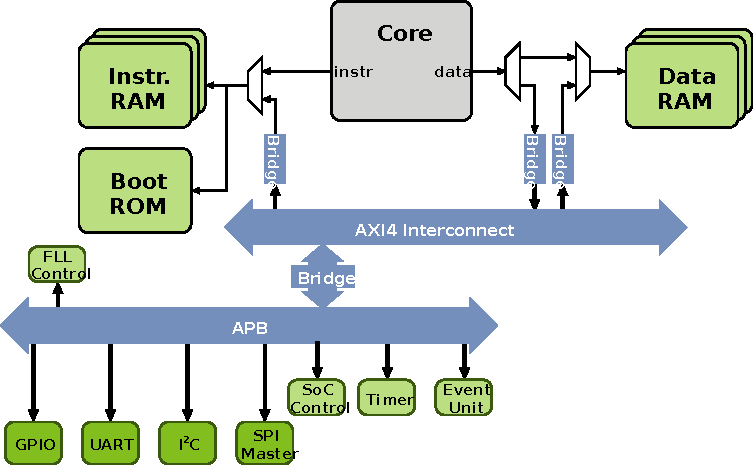
\includegraphics[width=\linewidth]{pdf/Pulp_complete.pdf}
        \caption{Arquitectura de la plataforma PULPino. }
        \label{fig:PULParch}
    \end{figure}
    





\end{document}

